\chapter{卒論っぽいサンプルその2}

\section{はじめに}
これから船体運動の運動方程式を説明していくが,その説明に際しては参考文献の書籍を参考にし,必要に応じて文章の表現を変えた.

\section{船の操縦運動の基本}
まず,船は通常スクリュープロペラ(プロペラと呼ぶ)を回転させることによって推力を発生させて前進し,船尾に装着された舵を動かすことによって船の針路変更が行われる.

舵は翼の一種であり,舵を切ることにより,揚力を発生させて,船を動かすのに必要な力を得る.一般に船の舵は船体と比べて非常に小さくなっているが,舵が船尾端に装着されることで舵力によるモーメントが大きくなり,小さくても十分に船を操舵できるのである.

そして,船の操縦運動の基本は,次の3つである.
\begin{enumerate}
	\item まっすぐ走る.
	\item 曲がる.
	\item 止まる.
\end{enumerate}

船において,決められた針路をまっすぐ走るための性能を針路安定性(course stability)という.この針路安定性が劣ると,舵を切っても応答性が悪くなり,右に左にふらふらしながら蛇行することになる.一般に,やせ型船と比較して,タンカーのような肥型船は,針路不安定になりやすいという傾向がある.

また,舵を切って船の針路を変える性能のことを,旋回性能(turning ability)と呼ぶ.旋回性能は,緊急回避するための重要な性能であり,より小さな半径で旋回できるほうがよい.

航行している船は,プロペラを逆転させて逆推力を発生させ,停止させる.この性能をプロペラ逆転停止性能(stopping ability)と呼ぶ.航走時から停止までの時間,距離は,小さいほどよい.

本研究ではこの3つのうち,(1)まっすぐ走る.と(2)曲がる.に焦点を当てていく.

\section{船の運動の呼び方}
船は3次元の剛体と考えることができる.そのとき,船に固定された座標系として,\figref{fig:2-1_png}のように,船の重心を原点にとり,船の長さ方向にx軸,横方向にy軸,上下(下向き)方向にz軸をとるのが一般的である.座標軸方向の運動を並進運動と呼び,それぞれ,

\begin{itemize}
	\item x軸方向の運動を前後運動(surge)
    \item y軸方向の運動を左右運動(sway)
    \item z軸方向の運動を上下運動(heave)
\end{itemize}

という.さらに,座標軸まわりの運動を回転運動と呼び,それぞれ,

\begin{itemize}
	\item x軸まわりの回転運動をロール運動(roll)
    \item y軸まわりの回転運動をピッチ運動(pitch)
    \item z軸まわりの回転運動を回頭運動(yaw)
\end{itemize}

という.

\begin{figure}[htbp]
    \centering   
    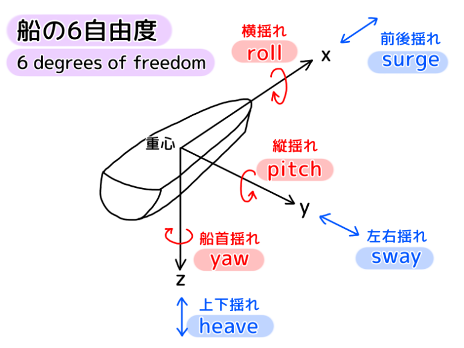
\includegraphics[width=0.8\textwidth]{./img/2-1.png}
    \caption{Degrees of freedom.}
    \label{fig:2-1_png}
\end{figure}

\section{基礎となる運動方程式}
基礎となる船の操縦運動方程式を導く.まず,船は剛体であると仮定する.また,波浪の影響はないものとし,平水中を操舵しながら航行する船の操縦運動を考える.従って,船の運動は平面運動内,すなわち,前後(surge),左右(sway),回頭(yaw)の3つの運動モードだけで定義される.

\begin{figure}[htbp]
    \centering   
    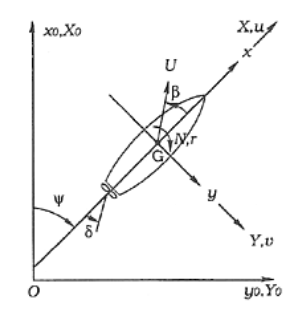
\includegraphics[width=0.8\textwidth]{./img/2-2.png}
    \caption{Degrees of freedom.}
    \label{fig:2-2_png}
\end{figure}

船体に作用する流体力等を計算する場合には,船体に固定された座標系で表す方が便利な方が多い.このため,\figref{fig:2-2_png}に示したような船に固定された座標系を考える.重心位置Gを原点に一致させ,船の前方にx軸方向を,船体横方向にy軸をとる.空間に対し鉛直下向きにz軸をとる.従って,x-y平面は静水面に対し平行となる.一方,空間に固定された座標系を考える.$X_0$-$Y_0$平面を静水面に一致させ,$Z_0$軸を鉛直下方にとる.$X_0$軸に対し,x軸のなす角度を方位角(heading angle)とし,$\Psi$と表す.なおFig. 2 2に示すように,船速を$U$,舵角を$\delta$,斜航角(drift angle)を$\beta$とする.
船の重心の速度を$\boldsymbol{V}$,方位に関する角速度とモーメントをそれぞれ$\boldsymbol{F},M_z$とする.太字で表された文字は,平面運動に関する2次元ベクトルを意味する.いま,$\boldsymbol{V},r,\boldsymbol{F},M_z$が慣性系で測られ,時刻$t$において,その座標系の原点が船体の重心に一致していたとする.この時船の運動方程式は次式で表される.

\begin{align}
    m \frac{d \boldsymbol{V}}{d t}=\boldsymbol{F} \label{eq:2-1} \\
    I_{z} \frac{d r}{d t}=M_{z} \label{eq:2-2}
\end{align}

ただし,$m$は船の質量,$I_z$は重心まわりの慣性モーメントである.
\equref{eq:2-1}に関する諸量を船体固定座標系について書き直す.$\boldsymbol{V}$を次のように表す.

\begin{align}
    \boldsymbol{V} &= u \boldsymbol{i} + v \boldsymbol{j} \label{eq:2-3}
\end{align}

なお,船速$U$は$abs(V)$と定義される.\equref{eq:2-3}において,$x$軸に関する単位ベクトルを$i$,$y$軸に関する単位ベクトルを$j$とする.そのとき,$i,j$と,$X_0$軸に関する単位ベクトル$i_0$,$Y_0$軸に関する単位ベクトル$j_0$との間には,次のような関係がある.

\begin{align}
    \boldsymbol{i} &= \cos{\Psi} \boldsymbol{i}_0 + \sin{\Psi} \boldsymbol{j}_0 \label{eq:2-4}\\
    \boldsymbol{j} &= - \sin{\Psi} \boldsymbol{i}_0 + \cos{\Psi} \boldsymbol{j}_0 \label{eq:2-5}
\end{align}

同様に,$\boldsymbol{F}$を次のように表す.

\begin{align}
    \boldsymbol{F} &= F_x \boldsymbol{i} + F_y \boldsymbol{j} \label{eq:2-6}
\end{align}

船体固定座標系において,運動方程式\equref{eq:2-1}は次のように表される.
\begin{align}
    \begin{split}
    m \frac{d \boldsymbol{V}}{d t}=m \frac{d(u \boldsymbol{i}+v \boldsymbol{j})}{d t} &=m\left(\frac{d u}{d t} \boldsymbol{i}+u \frac{d \boldsymbol{i}}{d t}+\frac{d v}{d t} \boldsymbol{j}+v \frac{d \boldsymbol{j}}{d t}\right) \\
    &=F_{x} \boldsymbol{i}+F_{y} \boldsymbol{j} \label{eq:2-7}
    \end{split}
\end{align}

式中,$\frac{d \boldsymbol{i}}{d t},\frac{d \boldsymbol{j}}{d t}$は\equref{eq:2-4}, \equref{eq:2-5}より,次のように表される.

\begin{align}
    \begin{split}
        \frac{d \boldsymbol{i}}{d t}&=\frac{d \cos \psi}{d t} \boldsymbol{i}_{0}+\frac{d \sin \psi}{d t} \boldsymbol{j}_{0} \\
        &=-r \sin \psi \boldsymbol{i}_{0}+r \cos \psi \boldsymbol{j}_{0}=r \boldsymbol{j} \label{eq:2-8}
    \end{split}
\end{align}

\begin{align}
    \begin{split}
        \frac{d \boldsymbol{j}}{d t}&=-\frac{d \sin \psi}{d t} \boldsymbol{i}_{0}+\frac{d \cos \psi}{d t} \boldsymbol{j}_{0} \\
        &=-r \cos \psi \boldsymbol{i}_{0}-r \sin \psi \boldsymbol{j}_{0}=-r \boldsymbol{i} \label{eq:2-9}
    \end{split}
\end{align}

ただし,$\frac{d\Psi}{d t}=r$である.

以上より,\equref{eq:2-7}は次のように書き換えられる.

\begin{align}
    m\left(\frac{d u}{d t} \boldsymbol{i}+u r \boldsymbol{j}+\frac{d v}{d t} \boldsymbol{j}-v r \boldsymbol{i}\right)=F_{x} \boldsymbol{i}+F_{y} \boldsymbol{j} \label{eq:2-10}
\end{align}

これを成分毎に表示すると

\begin{align}
    m(\dot{u} - vr) &= F_x \label{eq:2-11}\\
    m(\dot{v} + ur) &= F_y \label{eq:2-12}
\end{align}

となる.ここで,記号の上に付けた・は時間微分を意味する.

まとめると,船体固定座標系における船の操縦運動方程式は次のように表される.

\begin{align}
    \begin{split}
        m(\dot{u} - v r) &= F_x \\
        m(\dot{v} + u r) &= F_y \\
        I_z \dot{r} &= M_z \label{eq:2-13}
    \end{split}
\end{align}

\equref{eq:2-13}はスイスの数学者レオンハルト・オイラーが導いたことから,オイラーの運動方程式(Euler’s motion equations)と呼ばれる.未知数はu,v,rの3つであり,式の数3つと一致している.なお,式の操縦運動を扱う場合,uを前後速度,vを左右方向速度,rを回頭角速度と呼ぶ.

しかしながら,u,v,rが求まったとしても,船の位置や方位が得られたわけではない.それらは空間固定座標系に対する値として求める必要がある.ここで,船の重心の位置ベクトルを$\boldsymbol{R}$とする.

\begin{align}
    \boldsymbol{R} &= X_0 \boldsymbol{i}_0 + Y_0 \boldsymbol{j}_0 \label{eq:2-14}
\end{align}

これを時間tで微分すると速度ベクトルが得られ,これは船体固定座標系から見た速度ベクトルと等しくなるはずである.

\begin{align}
    \begin{split}
        \frac{d \boldsymbol{R}}{d t} &=\frac{d X_{0}}{d t} \boldsymbol{i}_{0}+\frac{d Y_{0}}{d t} \boldsymbol{j}_{0} \\
        &=u \boldsymbol{i}+v \boldsymbol{j} \label{eq:2-15}
    \end{split}
\end{align}

\equref{eq:2-4}, \equref{eq:2-5}を使って,\equref{eq:2-15}に含まれるi,jを書き換えると,次式が得られる.
\begin{align}
    \frac{d X_{0}}{d t} \boldsymbol{i}_{0}+\frac{d Y_{0}}{d t} \boldsymbol{j}_{0} &=  u (\cos{\Psi} \boldsymbol{i}_0 + \sin{\Psi} \boldsymbol{j}_0) + v (- \sin{\Psi} \boldsymbol{i}_0 + \cos{\Psi} \boldsymbol{j}_0) \label{eq:2-16}
\end{align}

これを成分毎に表示すると,

\begin{align}
    \frac{d X_{0}}{d t} &= u \cos \Psi - v \sin \Psi \label{eq:2-17}\\
    \frac{d Y_{0}}{d t} &= u \sin \Psi + v \cos \Psi \label{eq:2-18}
\end{align}

となる.この式は,船体固定座標系における速度成分と空間固定座標系における速度成分との関係を表す微分方程式である.これに$\frac{d \Psi}{d t}=r$という関係式を加えて,$X_0$,$Y_0$,$\Psi$に関する式がそろうことになる.

\section{船に作用する力とモーメント}

本節では,前節で述べた運動方程式における右辺の項,すなわち船に作用する力とモーメントについて考える.そのため基礎的な事項を説明し,具体的な表示式を示す.
\equref{eq:2-13}で表される運動方程式の外力成分$F_x,F_y,M_z$について考える.そのとき,$F_x,F_y,M_z$は,船の操縦運動(u,v,r)ならびに操船のための操作量である舵角$\delta$とプロペラ回転数$n_P$の計5つのパラメータの関数となる.すなわち,$F_x,F_y,M_z$はそれらの5つのパラメータを用いて,何らかの形で表示される.さらには,それらの時間微分の関数として表される可能性がある.それらを次のように表す.

\begin{align}
    \begin{split}
        F_{x} &=F_{x}\left(\dot{u}, \dot{v}, \dot{r}, u, v, r, \delta, n_{P}\right) \\
        F_{y} &=F_{y}\left(\dot{u}, \dot{v}, \dot{r}, u, v, r, \delta, n_{P}\right) \\
        M_{z} &=M_{z}\left(\dot{u}, \dot{v}, \dot{r}, u, v, r, \delta, n_{P}\right) \label{eq:2-19}
    \end{split}
\end{align}

$u,v,r$に関する船の流体力は,一般に,船の操縦運動を減衰させる方向に作用し,通常,抵抗や揚力と呼ばれる流体力成分からなる.よってそれらは,船が運動した結果によって発生した力とモーメントと考えられる.

$\dot{u},\dot{v},\dot{r}$に関する船の流体力は,船の運動加速度に比例する流体力成分,いわゆる付加質量,付加慣性モーメントと呼ばれる成分からなる.これについては,これから詳しく述べる.

$\delta$に関わる流体力は,いわゆる舵力であり,操縦運動を起こす源となる力とモーメントを意味する.本来ならば,$\delta$の時間微分,そしてこれをさらに時間微分した値も考慮しなければならないが,本論文では船の舵角は任意に与えることが出来るものとするので,舵の運動方程式は不要となる,従って,それらの値は考慮しないものとして扱う.

$n_P$にかかわる流体力は,いわゆるプロペラ推力のことであり,主に船の前後進運動を起こす源となる.直進航行時には,プロペラ推力によって発生する横力や回頭モーメントはほとんど0であり,前進力しか発生しないといえる一方で,プロペラ逆転時には,発生する横力や回頭モーメントは無視できない大きさとなる.しかし,本研究では逆転時のデータは扱っていないため,省略している.また,$n_P$に関しても,時間微分に比例した流体力成分が存在するが,プロペラ回転数は任意に与えることができるため,プロペラに関する運動方程式は不要となり,それらの値は考慮しないものとして扱う.

\subsection{付加質量}

付加質量とは,一般に,流体から受けた力があたかも質量が増加したように作用しているように見え,そのときの質量の増加分に相当するもののことを指す.

この付加質量は,対称性を持たない任意形状の物体であるとすると,$x$軸方向に加速すると,x軸方向だけでなく,$y$軸方向にも新たな付加質量が作用し,さらには$z$軸まわりの付加慣性モーメントが発生する.このことはこの物体が$y$軸方向に加速運動するとき,もしくは$z$軸まわりに回転運動するときにも同様である.

このように考えると船の付加質量(この言葉には,付加慣性モーメントも含む)には,船の前後運動(surge),左右運動(sway),回頭運動(yaw)に対して,それぞれ前後力,横力,回頭モーメントに関する3つの種類があることが分かる.いま,$i$の運動に対して,$j$に関する付加質量を$m_{ij}$と表す.ここで,$i=1,2,6$はそれぞれ前後運動(surge) ,左右運動(sway),回頭運動(yaw)を意味し,$j=1,2,6$はそれぞれ,前後力,横力,回頭モーメントを意味する.したがって,操縦運動に関する付加質量は,一般に,計$3×3=9$個の成分があることが分かる.ただし,船は左右対称であるため,前後運動に対し,横力や回頭モーメントは発生しない.すなわち$m_{12}=m_{16}=0$と言える.また,渦なしポテンシャル理論においては,$m_{ij}=m_{ji}$の関係があることが知られており,$m_{21}=m_{61}=0$とできる.なお$i=j$のときの付加質量を主要項と呼び,$i≠j$の付加質量を連成項と呼ぶ.まとめると,船の操縦運動を考えるときに必要な付加質量は,$m_{11},m_{22},m_{66}とm_{26}$の4つということになる.これらは,$m_x,m_y,J_z,m_y ,\alpha$($\alpha$は$m_y$の着力点と呼ばれるもの)と表されることが多い.この中で,$m_{26}$が前後対称であれば$0$となる.船はおおよそ前後対称であることが多いことから,$m_{26}$を$0$とすることが多い.本研究でも,$m_{26}$を$0$として取り扱う.

また,船に回転運動が伴う場合にはその回頭角速度に比例する形,すなわち,\equref{eq:2-13}の第1式と第2式の左辺第2項と同様な形で付加質量が作用する.これは,回転運動を伴うときには,速度と角速度に比例する形の付加質量が作用するためである.

以上をまとめると,\equref{eq:2-20}に示した船に作用する力とモーメントは次のように表すことができる.

\begin{align}
    \begin{split}
        F_{x}&=-m_{x} \dot{u}+m_{y} v r+X\left(u, v, r, \delta, n_{P}\right) \\
        F_{y}&=-m_{y} \dot{v}+m_{x} u r+Y\left(u, v, r, \delta, n_{P}\right) \\
        M_{z}&=-J_{z} \dot{r}+Z\left(u, v, r, \delta, n_{P}\right) \label{eq:2-20}
    \end{split}
\end{align}

\section{船に作用する流体力の数学モデル}

次に,\equref{eq:2-20}中に現れる$X,Y,N$の表示について考えていく.$X,Y,N$の具体的な表示式の事を数学モデルと呼ぶ.$X,Y,N$は,船の操縦運動$(u,v,r)$ならびに操船のための操作量,すなわち舵角$\delta$とプロペラ回転数$n_P$の計5つの関数となる.それらの表示式は,船の運動や操作量の関数として,できるだけ簡単に表されることが望ましい.そこで,種々の仮定を設けて,流体力の簡略化を図る.簡略化に際しては,いくつかの係数を導入し,それによって流体力特性の特徴を代表させ,その係数は実験的に求めることができるものとする.

操舵時における舵の接線方向の流体力やプロペラに作用する横力成分を無視すると,$X,Y,N$は具体的に以下のように表示される.

\begin{align}
    X\left(u, v, r, \delta, n_{P}\right) &\cong X_{H}(u, v, r)-R_{0}(u)+\left(1-t_{P}\right) T_{P}\left(u, v, r, n_{P}\right) - \left(1-t_{R}\right) F_{N}\left(u, v, r, \delta, n_{P}\right) \sin \delta  \label{eq:2-21} \\
    Y\left(u, v, r, \delta, n_{P}\right) &\cong Y_{H}(u, v, r)+\left(1+a_{H}\right) F_{N}\left(u, v, r, \delta, n_{P}\right) \cos \delta  \label{eq:2-22} \\
    N\left(u, v, r, \delta, n_{P}\right) &\cong N_{H}(u, v, r)+\left(x_{R}+a_{H} x_{H}\right) F_{N}\left(u, v, r, \delta, n_{P}\right) \cos \delta \label{eq:2-23}
\end{align}

各項は次のような意味を持つ.

\begin{description}
    \item[$R_0$]直進時の船体抵抗
    \item[$X_H$]斜航,旋回時の船体に作用する前後方向の流体力変化
    \item[$Y_H, N_H$]斜航,旋回時の船体に作用する横力と回頭モーメント
    \item[$T_P$]プロペラ推力
    \item[$t_P$]推力減少率
    \item[$F_N,x_R$]舵直圧力ならびにその作用点の座標値
    \item[$t_R$]操舵による船体抵抗の減少ならびにプロペラ推力の増加を表す係数
    \item[$a_H, x_H$]操舵によって船体に誘起される横力成分の増加率とその着力点の座標値
\end{description}

\equref{eq:2-21}右辺第1項と第2項は主船体に作用する流体力,第3項はプロペラ推力$X_P$に関する項,第4項は操舵による舵抵抗増加$X_R$を意味する.プロペラ作動による船体抵抗の変化や舵抵抗の増加といった干渉流体力の項は,自航要素にならい推力減少率$t_P$を,同様に$t_R$をという係数を導入して表示する.\equref{eq:2-22}と\equref{eq:2-23}の右辺第1項は主船体に作用する横力と回頭モーメント,第2項は操舵によって発生する横力と回頭モーメントを意味する.船体と舵との干渉によって船体に付加される横力と回頭モーメントは,$a_H$と$x_H$の導入により,舵力の一部として考える.主船体に作用する流体力$(X_H,Y_H,N_H )$は,プロペラや舵との干渉流体力成分を含まない点に注意する.

これらの数学モデルはMMG(Maneuvering Modeling Group)モデルと呼ばれる.ただし,MMGモデルとはモデルの骨格のことであり,舵力やプロペラ推力等の具体的な表示はを規定したものではない. また,MMGモデルは船全体に働く流体力を船体,プロペラ,舵のそれぞれ単体に働く成分とそれらの相互間に生ずる干渉項とに分離して表しているため,外力があってプロペラの作動状態が通常と大きく異なる場合などの部分的な変化に容易に対応できる.

MMGモデルに必要な入力情報\tbref{tb:2-1}に示す情報であり、それらについて,これから具体的な表示式を示していく.本研究では操縦運動モデルとしてrefを参考にした一般的なMMGモデルを使用する.

\begin{table}[htbp]
 \caption{The data required for MMG}
 \label{tb:2-1}
 \centering
  \begin{tabular}{llll}
    \multicolumn{2}{c}{船体情報} & \multicolumn{2}{c}{操縦性能} \\
    \hline
    \hline
    $L$ & 船長$L_{pp}$[m] & $C_1$ & \multirow{3}{*}{スラスター係数} \\
    $B$ & 船幅[m] & $C_2$ \\
    $d$ & 喫水[m] & $C_3$ \\
    $Cb$ & 方形係数[-] & $X_0$ & \multirow{17}{*}{操縦流体力微係数} \\
    $m\_$ & 質量(無次元化)[-] & $X_{\beta \beta}$ \\
    $I_{z}$ & 慣性モーメント[-] & $X_{\beta \gamma}$ \\
    $t_P$ & 推力減少率 & $X_{\gamma \gamma}$ \\
    $w_{P0}$ & 有効伴流率 & $X_{\beta \beta \beta \beta}$ \\
    $m_x$ & 付加質量 $x$(無次元) & $Y_{\beta}$ \\
    $m_y$ & 付加質量 $y$(無次元) & $Y_{\gamma}$ \\
    $J_{z}$ & 付加質量 $I_z$(無次元) & $Y_{\beta \beta \beta}$ \\
    $t_R$ & 操縦抵抗減少率 & $Y_{\beta \beta \gamma}$ \\
    $a_H$ & 舵力増加係数 & $Y_{\beta \gamma \gamma}$ \\
    $x_H$ & 舵力増分作用位置 & $Y_{\gamma \gamma \gamma}$ \\
    $\gamma_R$ & 整流係数 & $N_{\beta}$ \\
    $l_r$ & 船長に対する舵位置 & $N_{\gamma}$ \\
    $\kappa$ & 修正係数 & $N_{\beta \beta \beta}$ \\
    $k_x$ & 流速増加修正係数 & $N_{\beta \beta \gamma}$ \\
    $\epsilon$ & プロペラ・舵位置伴流係数比 & $N_{\beta \gamma \gamma}$ \\
    $D_p$ & プロペラ直径[m] & $N_{\gamma \gamma \gamma}$ \\
    $H_R$ & 舵高さ[m] \\
    $A_R \_ L_d$ & 船の断面に対する舵面積比[-] \\
    $\Lambda$ & アスペクト比[-]
  \end{tabular}
\end{table}

\subsection{直進時の船体抵抗}

直進航行時の船体抵抗の表記については,船の推進性能の分野で用いられる方法をそのまま用いる.そこには,3次元外挿法と呼ばれるものと2次元外挿法と呼ばれる2つのものがある.

3次元外挿法では,相当平板の摩擦抵抗係数$C_f$に,形状影響係数$K_f$,造波抵抗係数$r_w$を用いて,次式で計算する.

\begin{align}
    \begin{split}
        R_{0}&=\rho \nabla^{2 / 3} u^{2}\left[(1 / 2)\left\{C_{f}\left(1+K_{f}\right)+\Delta C_{f}\right\} S / \nabla^{2 / 3}+r_{w}\right] \\
        C_{f}&=0.066 /\left\{\log _{10}\left(R_{e}\right)-2.03\right\}^{2} \label{eq:2-24}
    \end{split}
\end{align}

ここで,$\nabla$は船の排水容積,$S$は船の浸水面積,$R_e$はレイノルズ数である.$r_w$は$\nabla^{\frac{2}{3}}$をベースに無次元化されており,通常,水線長$L_{wl}$をベースとしたフルード数によって整理される.$\Delta C_f$は粗度修正係数である.\equref{eq:2-24}の第2式はHughesの式と呼ばれるものであるが,種々の式が提案されており,それらの式を適宜使用する.

2次元外挿法では,相当平板の摩擦抵抗係数$C_f$に,剰余抵抗係数$r_R$を用いて,次式で計算する.


\begin{align}
    \begin{split}
        R_{0}&=\rho \nabla^{2 / 3} u^{2}\left[(1 / 2)\left\{C_{f} +\Delta C_{f}\right\} S / \nabla^{2 / 3}+r_{R}\right] \\
        C_{f}&=0.075 /\left\{\log _{10}\left(R_{e}\right)-2\right\}^{2} \label{eq:2-25}
    \end{split}
\end{align}

\equref{eq:2-25}の第2式はITTC1957年の式と呼ばれるものであるが,種々の式が提案されており,上と同様に,それらを適宜使用する.

\subsection{斜航・旋回時の船体に作用する流体力}

船が斜航したり,旋回するときに船体に作用する流体力は,主に流体の動圧によって生じると考えられる.もし船の幅が小さいと考えられるのならば,船体はコード長を船長$L$に,スパン長を喫水$d$にとった小アスペクト比翼とも考えることができる.そのとき翼面積にあたるパラメータは$L d$となる.以上のような考察の下,船体に作用する流体力$(X_H,Y_H,N_H )$は次式で表される

\begin{align}
    \begin{split}
        X_{H} &=(1 / 2) \rho L d U^{2} X_{H}^{\prime}\left(\beta, r^{\prime}\right) \\
        Y_{H} &=(1 / 2) \rho L d U^{2} Y_{H}^{\prime}\left(\beta, r^{\prime}\right) \\
        N_{H} &=(1 / 2) \rho L d U^{2} N_{H}^{\prime}\left(\beta, r^{\prime}\right) \label{eq:2-26}
    \end{split}
\end{align}

式中,$U$は合速度であり,$U\equiv\sqrt{u^2+v^2}$と定義される.
${X^{\prime}}_H, {Y^{\prime}}_H, {N^{\prime}}_H$が流体力係数に相当する.
なお,$´$ は無次元値であることを意味する.この流体力係数は,船の斜航角$\beta$と無次元化された回頭角速度$r^{\prime}(\equiv \frac{rL}{U})$  だけの関数としており,船速に無関係である.これは流体力係数に及ぼす造波の影響を無視したことを意味する.
水槽試験結果より,${X^{\prime}}_H$は$\beta$と$r^{\prime}$に関して偶関数であり,${Y^{\prime}}_H,{N^{\prime}}_H $は奇関数であることが知られている.これを踏まえて,${X^{\prime}}_H, {Y^{\prime}}_H, {N^{\prime}}_H$を$\beta,r^{\prime}$のべき多項式で表すことを考える.${X^{\prime}}_H$は偶関数であることから,1次の項を省略し,${Y^{\prime}}_H,{N^{\prime}}_H$は奇関数であることから2次の項を省略することとする.すると,${X^{\prime}}_H,{Y^{\prime}}_H,{N^{\prime}}_H$は次に示すような多項式で表される.


\begin{align}
    \begin{split}
        X_{H}^{\prime}\left(\beta, r^{\prime}\right)&=X_{0}^{\prime}+X_{\beta \beta}^{\prime} \beta^{2}+X_{\beta r}^{\prime} \beta r^{\prime}+X_{r r}^{\prime} r^{\prime 2}+X_{\beta \beta \beta \beta}^{\prime} \beta^{4} \\
        Y_{H}^{\prime}\left(\beta, r^{\prime}\right)&=Y_{\beta}^{\prime} \beta+Y_{r}^{\prime} r^{\prime}+Y_{\beta \beta r}^{\prime} \beta^{2} r^{\prime}+Y_{\beta r r}^{\prime} \beta r^{\prime 2}+Y_{\beta \beta \beta}^{\prime} \beta^{3}+Y_{r r r}^{\prime} r^{\prime 3} \\
        N_{H}^{\prime}\left(\beta, r^{\prime}\right)&=N_{\beta}^{\prime} \beta+N_{r}^{\prime} r^{\prime}+N_{\beta \beta r}^{\prime} \beta^{2} r^{\prime}+N_{\beta r r}^{\prime} \beta r^{\prime 2}+N_{\beta \beta \beta}^{\prime} \beta^{3}+N_{r r r}^{\prime} r^{\prime 3} \label{eq:2-27}
    \end{split}
\end{align}

式中の${X^{\prime}}_{\beta \beta}$,${X^{\prime}}_{\beta r}$,${X^{\prime}}_{r r}$,${X^{\prime}}_{\beta\beta\beta\beta}$,${Y^{\prime}}_{\beta}$,${Y^{\prime}}_{r}$,${Y^{\prime}}_{\beta \beta \beta}$,${Y^{\prime}}_{\beta \beta r}$,${Y^{\prime}}_{\beta r r}$, ,${Y^{\prime}}_{r r r}$,${N^{\prime}}_{\beta}$,${N^{\prime}}_{r}$,${N^{\prime}}_{\beta \beta \beta}$,${N^{\prime}}_{\beta \beta r}$,${N^{\prime}}_{\beta r r}$, ,${N^{\prime}}_{r r r}$は操縦流体力微係数と呼ばれる.また,βやr'に比例する微係数は線形微係数,それ以外は非線形微係数と呼ばれる.

ここでは,${X^{\prime}}_H$は$\beta$と$r^{\prime}$に関する2次+4次形式,${Y^{\prime}}_H$, ${N^{\prime}}_H$は1次+3次形式の表示式とした.一般に,この多項式の次数は適宜決めることができる.したがって,今回も\equref{eq:2-27}のような表示式にした.多項式の次数を増やすと,流体力特性の近似精度は向上するが,増やしすぎると取り扱いが面倒になるので,実用上は3,4次程度が妥当である.

\subsubsection{干渉流体力係数}

\equref{eq:2-21}, \equref{eq:2-22}, \equref{eq:2-23}で用いられる$t_P,t_R,a_H,x_H$は,船体とプロペラ,船体と舵に関する干渉を表す係数である.それら干渉流体力係数について説明する.

$t_P$は推力減少率と呼ばれ,プロペラが作動することによって,船体の圧力分布が変化し,船体抵抗や舵抵抗が増加することを表す係数である.これは,船の推進性能を議論するときによく知られたものである.$t_P$は,一般にプロペラ荷重度によって変化するが,操縦運動に伴う荷重度の変化に対しては,一定値として取り扱われることが多い.

$t_R$は操舵抵抗減少率と呼ばれ,舵直圧力$F_N$の船長方向成分,$F_N  \sin{\delta}$に対する減少率として表される.物理的には,操舵によって生じる船体抵抗減少ならびに操舵に伴うプロペラ推力の増加を意味する.後者は,操舵によって,プロペラ位置での伴流が増加し,プロペラ推力が増加することによって生じる.一方,前者については,操舵によって船体抵抗が減少するというメカニズムが,今のところ,不明である.\equref{eq:2-21}, \equref{eq:2-22}, \equref{eq:2-23}から分かるように,基礎となる式において,舵の接線方向流体力成分が無視されており,その影響がこのような形で表れているとも考えられる. 
$a_H$と$x_H$は,それぞれ舵力増加係数,舵力増分作用位置と呼ばれ,操舵によって船体に誘起される横力成分の増加率とその着力点を意味している.$a_H$は舵直圧力の船体横方向成分$F_N  \cos{\delta}$に対する増加率として表される.この現象は,主翼を船体,フラップ翼を舵とみなすと,理解が容易である.すなわち,舵を切ると舵に直圧力が発生するが,それと同時に,船体にもあらたな横力が発生することになる.これは,主翼とフラップ翼に作用する流体力の減少と同じ原理に基づく.

なお,$t_R,a_H,x_H$は,一般に,操縦運動$(u,v,r)$や操作量$(\delta,n_P )$の関数になると考えられるが,そのような取り扱いはあまりに煩雑であるため,単に定数として取り扱うことが多い.このような取り扱いでも実用上十分とされる.$t_R,a_H,x_H$の値は水槽試験で求めることができ,おおよそ次のような大きさとなる.

\begin{itemize}
	\item $t_R$は0.25程度の値をとる.
	\item $a_H$は方形係数$C_b$とともに大きくなる傾向があり,平均的には0.5程度の値となる.
	\item ${X^{\prime}}_H (=\frac{x_H}{L})$ は $C_b$ に関わらず-0.45ぐらいの値をとる.AP位置は-0.5であることから,APよりもやや前方付近に干渉横力成分が誘起されることが分かる.
\end{itemize}

\subsubsection{プロペラ推力}
プロペラは,回転する翼と考えられるので,プロペラ推力$T_P$は速度の二乗とプロペラ作動面積に比例する.速度として,プロペラ先端の円周速度$\pi n_P  D_P$($n_P$はプロペラ回転数,$D_P$はプロペラ直径)をとり,面積としてプロペラ面の円面積をとると,推力$T_P$は$T_P \propto \rho (n_P D_P)^2 {D_P}^2 = \rho {n_P}^2 {D_P}^4$となる.比例定数を$K_T$とすると,

\begin{align}
    \begin{split}
        T_P &= K_T \rho {n_P}^2 {D_P}^4 \label{eq:2-28}
    \end{split}
\end{align}

で表される.$K_T$はスラスト係数といい,前進常数$J$の関数として表される.$J$は次のように定義される.

\begin{align}
    \begin{split}
        J &= \frac{u(1-w_P)}{n_P D_P} \label{eq:2-29}
    \end{split}
\end{align}

$K_T$は前進常数Jをベースとして,次式のように表す方法が広く用いられている.

\begin{align}
    \begin{split}
        K_T &= C_1 + C_2 J + C_3 J^2 \label{eq:2-30}
    \end{split}
\end{align}

ここで,$C_1,C_2,C_3$は$K_T$ の特性を表すスラスター特性係数である.一般的にスラスター特性係数$C_1,C_2,C_3$はプロペラ単独性能試験より算出される.

前進常数Jを表す\equref{eq:2-29}において,$w_P$は有効伴流率とよばれ,プロペラに流入する速度の減速率を表す.プロペラは,通常,船の後ろにできる遅い流れの中で作用するので,$w_P$は0よりも大きな値をとる.この$w_P$は船の操縦運動とともに変化し,一般に,操縦運動の発達とともに,船尾での船速が加速され,$w_P$は小さくなる傾向がある.

\subsection{舵力}

舵は翼の一種であり,舵力は流体力学でいう揚力と考えられる.これから3次元平板翼の揚力係数について考える.

\subsubsection{3次元平板翼の揚力係数}
3次元の平板翼は揚力線理論を用いると,3次元平板翼の揚力係数$C_L$は次のように表される.

\begin{align}
    \begin{split}
        C_{L}=\frac{2 \pi \Lambda}{\Lambda+2} \alpha \label{eq:2-31}
    \end{split}
\end{align}

ここで,$\alpha$は迎角,$\Lambda$は翼のアスペクト比である.アスペクト比とは,翼面積を$A_w$,スパン長を$b$とするとき,

\begin{align}
    \begin{split}
        \Lambda &= \frac{b^2}{A_w} \label{eq:2-32}
    \end{split}
\end{align}

と定義されるもので、,$A_w=b c$($c$はコード長)で計算できる矩形翼の場合には,単に$\Lambda=\frac{b}{c}$と表されるため,縦横比とも呼ばれる.アスペクト比は翼の性能を決める重要なパラメータである.

3次元翼の揚力勾配係数を改めて$f_{\alpha}$と書くと,

\begin{align}
    \begin{split}
        f_{\alpha}=\frac{2 \pi \Lambda}{\Lambda+2} \label{eq:2-33}
    \end{split}
\end{align}

となる.この式は,揚力線近似モデルが採用されているうえに,循環が楕円翼循環分布で表されるという仮定の下で誘導された式であることに注意が必要である.

\subsubsection{舵直圧力の数学モデル}

以上を踏まえ,舵直圧力$F_N$の数学モデルを考える.$F_N$は翼に作用する揚力とみなすことができるため,次のように表すことができる.

\begin{align}
    \begin{split}
        F_N &= \frac{1}{2} \rho A_R {U_R}^2 f_\alpha \sin{\alpha_R} \label{eq:2-34}
    \end{split}
\end{align}

式中,$A_R$は舵面積,$f_\alpha$は舵直圧力勾配係数,$U_R$は舵への流入速度,$\alpha_R$は舵への流入速度である.舵は船体後方の伴流域のプロペラ後流中に存在する.従って,$U_R$と$\alpha_R$をいかに合理的に表示するかが鍵となる.なお,$f_\alpha \sin{α_R} $の部分が揚力係数($C_L$ )に相当する.$U_R$と$\alpha_R$は次式で表される.

\begin{align}
    U_R &= \sqrt{{u_R}^2 + {v_R}^2} \label{eq:2-35} \\
    \alpha_R &= \delta - \tan^{-1}{\frac{v_R}{u_R}} \label{eq:2-36}
\end{align}

$u_R$は舵に流入する前後方向の速度成分,$v_R$はプロペラ後流中での横方向速度成分である.

\subsubsection{直圧力勾配係数}

直圧力勾配係数$f_\alpha$は\equref{eq:2-37}で表される揚力勾配係数を使用しておおよそ推定できる.なお,日本では,この揚力線理論解をベースとして,水槽試験結果と良い一致を示すように修正を施した式が広く用いられており,それは次のように表される. 

\begin{align}
    f_\alpha &= \frac{6.13 \Lambda}{\Lambda + 2.25} \label{eq:2-37}
\end{align}

\equref{eq:2-33}と\equref{eq:2-37}はよく似たものとなっていることが分かる. 

\equref{eq:2-37}を用いて,種々のアスペクト比における舵角$\delta$に対する揚力係数$C_L$ ($=f_\alpha \sin{\alpha_R} $)を計算する.アスペクト比Λが大きくなるほど,迎角(舵角) $\delta$に対する傾きが大きくなる.一様流中の翼(舵)では,揚力係数が1.2~1.4になると,失速が起こり,それ以上に揚力係数は大きくならないという現象が起こる.しかし,実際の舵は,船体後方のプロペラ後流中という不均一な流れの中にあるため,舵角が35degのような大きな場合があっても,失速は起きないと考えて差し支えない.従って,アスペクト比の大きな舵ほど性能的には有利になるが,実際には船の喫水によって舵高さは制限され,船種および船の大きさによっては舵面積比がほぼ決定されるため,採用される舵のアスペクト比は,1~2程度の値に制限されることになる.

\subsubsection{舵に流入する横方向速度成分}
舵に流入する横方向成分$v_R$を考えるとき,留意すべきことは,船の操縦運動による影響をいかに考慮するかである.

$v_R$は,舵位置での船の操縦運動による幾何学的な流入角$\beta_R$ ($\equiv \beta-{l^{\prime}}_R  r^{\prime}$)に整流効果を表す係数$\gamma_R$を導入した式で表す.

\begin{align}
    v_R &= U \gamma_R (\beta - {l^{\prime}_R} r^{\prime}) \label{eq:2-38}
\end{align}

式中,$\gamma_R$は整流係数と呼ばれる.整流係数は,$\beta_R$に比例する係数であり,通常1.0よりも小さな値を取る.すなわち,舵に流入する角度は,船体ならびにプロペラの影響により,船の長さ方向に流れに近づくように整流され,船の操縦運動による幾何学的な角度よりも小さくなることを意味する.$\beta_R$は,船体斜航角$\beta$と船が回頭することによる舵位置での流入変化$-{l^{\prime}}_R  r^{\prime}$の和で表される.この場合,${l^{\prime}}_R $は舵位置の座標を船長Lで割って無次元化したものであり,本来-0.5とすべきものである.しかし実際に,${l^{\prime}}_R $を実験的に求めてみると,${l^{\prime}}_R \simeq 1.0 $であったため,今では,${l^{\prime}}_R $は,本来の意味では使用されずに,単なる実験定数として捉えられるようになっている.整流係数$\gamma_R$は操縦運動に大きな影響を及ぼすため,操縦運動のシミュレーション計算等において,正しく把握する必要がある.また,右旋回と左旋回において,整流係数が異なる値を取ることが知られており,旋回航跡が左右非対称となる理由の1つとなっている.左右旋回運動における平均の整流係数$\gamma_R$と${l^{\prime}}_R $はそれぞれ0.45,-0.9程度の値となる.

\subsubsection{舵に流入する前後方向速度成分}

舵はプロペラ後流中で作動することを特徴とする.従って,舵に流入する前後方向速度成分$u_R$を考えるときには,プロペラ作動の影響をいかに含ませるかという点がポイントとなる.まず,$u_R$は次式で表されると仮定する.

\begin{align}
    \begin{split}
        v_{R}&=\sqrt{\frac{A_{R 1}}{A_{R}} u_{R P}^{2}+\frac{A_{R 2}}{A_{R}} v_{R 0}^{2}} \\
        &=\sqrt{\eta_{R} u_{R P}^{2}+\left(1-\eta_{R}\right) v_{R 0}^{2}} \label{eq:2-39}
    \end{split}
\end{align}


この式は,舵にプロペラの後流があたる部分の流速$u_{RP}$とあたらない部分の流速$u_{R0}$の2つを考えて,それぞれの流入面積を考慮し加重平均値をとるとしたものである.ここで,$A_{R1}$はプロペラ後流があたる部分の舵面積,$A_{R2}$はプロペラ後流があたらない部分の舵面積,$A_R$は全舵面積(すなわち,$A_R=A_{R1}+A_{R2}$)を意味する.$\eta_R$は

\begin{align}
    \begin{split}
        \eta_R &= \frac{A_{R1}}{A_R} \simeq \frac{D_P}{H_R} \label{eq:2-40}
    \end{split}
\end{align}

を意味し,プロペラ直径$D_P$と舵高さ$H_R$から計算されることが多い.
$u_{R0}$はプロペラ後流の影響を考慮しない舵位置での伴流係数$w_R$を定義して,次のように表す.

\begin{align}
    u_{R0} &= (1-w_R) u \label{eq:2-41}
\end{align}

また,$u_{RP}$は

\begin{align}
    u_{RP} &= u_{R0} + k_x \Delta u \label{eq:2-42}
\end{align}

と表す.ここで$k_x \Delta u$がプロペラ後流の影響による流速増加を表す.$\Delta u$は後述する理論的な流速増加であり,$k_x$はその修正係数である.$\Delta u$は無限後方位置での流速$u_\infty$とプロペラへの流入速$u_P$との差と定義する(すなわち$\Delta u = u_\infty-u_P$).なお,$u_P$はプロペラ位置での有効伴流率$w_P$を用いて,$u_P=(1-w_P )u$と表すことができる.$u_\infty$と$u_P$の間には,プロペラ前後の圧力差を$\Delta p$とするとき,ベルヌーイの定理より次のような関係がある.

\begin{align}
    \Delta p + \frac{\rho}{2} {u_P}^{2} &= \frac{\rho}{2} {u_\infty}^{2} \label{eq:2-43}
\end{align}

なお,$\Delta p$とプロペラ推力$T_P$との間には,

\begin{align}
    T_P &= \Delta p \pi (\frac{D_P}{2})^2 \label{eq:2-44}
\end{align}

という関係がある.加えて,\equref{eq:2-28}の関係を考慮すると,$u_\infty$は,

\begin{align}
    u_\infty &= u_P \sqrt{1+\frac{8 K_T}{\pi J^2}} \label{eq:2-45}
\end{align}

と表すことができる.

\equref{eq:2-39}に,\equref{eq:2-41}\equref{eq:2-42}を代入し,\equref{eq:2-45}等を用いて,$\Delta u$や$u_\infty$を消去すると,\equref{eq:2-46}が得られる.


\begin{align}
    u_{R}=\varepsilon_{w} u_{P} \sqrt{\eta_{R}\left\{1+\kappa\left(\sqrt{1+\frac{8 K_{T}}{\pi J^{2}}}-1\right)\right\}^{2}+\left(1-\eta_{R}\right)} \label{eq:2-46}
\end{align}

ここで,$\epsilon_w$はプロペラ・舵位置伴流係数比と呼ばれ,舵位置での伴流係数とプロペラ位置での伴流係数の比を意味し,$\epsilon_w=\frac{1-w_R}{1-w_P}$と定義される.
また,$\kappa$は$\frac{k_x}{\epsilon_w}$ と定義される修正係数である.
この式は,$\epsilon_w$と$\kappa$(もしくは$k_x$)を決めることができれば,プロペラ推力特性やプロペラ直径と舵高さの影響等が含まれた形で,舵への流入速度を決めることができる.通常,$\epsilon_w$は1.1程度,$k_x$は0.6程度の値になるといわれるが,舵の種類や船尾形状によっても変化する.

\subsection{船に作用する横力と回頭モーメントの線形表示}

以上,船に作用する流体力の数学モデルについて述べた.ここでは,その表示形式をベースに,操縦運動v,rや舵角$\delta$は微小との仮定の下,船に作用する横力と回頭モーメントを簡略化し,$v,r,\delta$に関する線形の表示式を求める.そのときの$v,r,\delta$に対する比例係数を線形微係数と呼ぶ.なお,船は船速$U$で航走しているものとし,前後方向の流体力については議論しない.また,2次以上の微小項については省略して考える.

ここでは,舵直圧力$F_N$の線形化を考える.$\sin{\delta} \simeq \delta, \cos{\delta} \simeq 1$であることに注意すると,\equref{eq:2-34}において,$U_R$は$u_R$に,$\sin{\alpha_R}$は$\alpha_R$と近似されるので,

\begin{align}
    \begin{split}
        F_N &= \frac{1}{2} \rho A_R {U_R}^2 f_\alpha \alpha_R  \label{eq:2-47}
    \end{split}
\end{align}

が得られる.さらに$\alpha_R$は\equref{eq:2-36}\equref{eq:2-38}より

\begin{align}
    \begin{split}
        \alpha_R &\cong \delta - \frac{v_R}{u_R} \\
        &= \delta + \frac{U (v^{\prime}) + {l^{\prime}}_R r^{\prime}}{u_R} \gamma_R \label{eq:2-48}
    \end{split}
\end{align}

と表されるので($\beta=-v^{\prime}$ であることに注意),結局$F_N$は次のように表示される.

\begin{align}
    \begin{split}
        \mathrm{F}_{N} \cong(1 / 2) \rho A_{R} u_{R}^{2} f_{\alpha}\left[\delta+\frac{U\left(v^{\prime}+l^{\prime}_{R} r^{\prime}\right)}{u_{R}} \gamma_{R}\right] \label{eq:2-49}
    \end{split}
\end{align}

両辺を$\frac{1}{2} \rho L d U^2$で割って無次元化すると,

\begin{align}
    \begin{split}
        \mathrm{F}_{N}^{\prime} \cong \frac{A_{R}}{L d} f_{\alpha}\left[u_{R}^{\prime}{ }^{2} \delta+u_{R}^{\prime} \gamma_{R}\left(v^{\prime}+l_{R}^{\prime} r^{\prime}\right)\right] \label{eq:2-50}
    \end{split}
\end{align}

が得られる.なお,$u^{\prime}_R=\frac{u_R}{U}$である.$u^{\prime}_R$は$v$や$r$によって変化する可能性があるが,ここではそのままの形で残すことにする.
ここで,導いた表示形式は推定にというよりはシミュレーションの際に適宜使用する.

\section{旋回性能}

本節では,操縦性能のうち最も代表的な性能である旋回性能について考える.旋回運動の基礎について述べた後,数値的に旋回運動を求めるための計算法について述べる.

\subsection{旋回運動発達の概論}
優れた旋回性能というのは,いわば操舵に対して「小回りが効く」ということであり,船の長さに対する旋回航跡の大きさが一つの尺度になる.旋回航跡の表現には,以下に示すような代表的な数値が伝統的に使用されている.Fig. 2 3を用いて説明する.

方位角が原針路から90degに達するまでの進出距離(操舵開始後から原針路方向に進む距離)を縦距($D_A$),また,その時点の横方向の移動距離を横距($D_t$)という.また,船が原針路から反転して180degに達した時点の横方向の移動距離を旋回圏($D_T$)と呼ぶ.
船は旋回運動と同時に横流れ運動も生じているので,最大縦距や最大横距は90deg旋回時点ではなく,そのあと遅れて発生する.最大旋回圏も同様である.
また,操舵直後に発生する旋回方向と逆の移動をキックと言い,この大きさは船の幅の数\%と比較的小さいが,船尾位置におけるキック(キックアウト)は必ずしも小さくないので,狭い港湾域の操船では注意を要する.

\begin{figure}[htbp]
    \centering   
    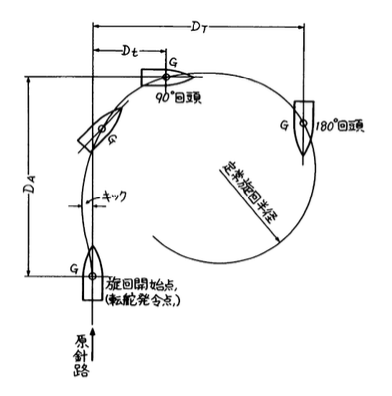
\includegraphics[width=0.8\textwidth]{./img/2-3.png}
    \caption{The image on ship turning.}
    \label{fig:2-3_png}
\end{figure}

\subsection{旋回運動の数値計算}

前節で述べた旋回運動に関する諸式は,舵角が小さく操縦運動が微小の場合において有効である.しかし,舵角35degといった大舵角を考える場合には,舵力をはじめ船体に作用す流体力の非線形影響が強くなり,旋回運動特性を解析的に求めることはできない.その場合に,旋回運動特性を正しく求めるには,数値的な解法に頼らざるを得ない.ここでは,旋回運動の数値計算法について述べる.

\subsubsection{運動方程式}

まず,基礎となる運動方程式を整理する.\equref{eq:2-13}に\equref{eq:2-30}を代入すると,次式が得られる.

\begin{align}
    \begin{split}
        \left(m+m_{x}\right) \dot{u}+\left(m+m_{y}\right) v r&=X \\
        \left(m+m_{y}\right) \dot{v}+\left(m+m_{x}\right) u r&=Y \\
        \left(I_{z}+J_{z}\right) \dot{r}&=N \label{eq:2-51}
    \end{split}
\end{align}

船に作用する流体力$X,Y,N$は次のように表す.

\begin{align}
    \begin{split}
        X &= X_H - R_0 + X_R + X_P \\
        Y &= Y_H + Y_R \\
        N &= N_H + N_R \label{eq:2-52}
    \end{split}
\end{align}

上式内の右辺は\equref{eq:2-21}\equref{eq:2-22}\equref{eq:2-23}の第1項,第2項(Xのみ第3項と第4項も)に対応している.

\subsubsection{旋回運動の時刻歴計算法}

次に,旋回運動の時刻歴計算法について述べる.解くべき微分方程式は,\equref{eq:2-51}であり,\equref{eq:2-52}を用いて,それを書き換えると次のようになる.

\begin{align}
    \begin{split}
        \dot{u} &= \frac{X_H - R_0 + X_R + X_P + (m + m_y) v r}{m + m_x} \\
        \dot{v} &= \frac{Y_H + Y_R - (m + m_x) u r}{m + m_y} \\
        \dot{r} &= \frac{N_H + N_R}{I_z + J_z} \label{eq:2-53}
    \end{split}
\end{align}

これを数値的に解くことを考える.

数値解法として,オイラー法,ルンゲ・クッタ法,予測子修正子法などの方法があるが,ここでは最も簡単なオイラー法について説明する.

$(u,v,r)\equiv(x_1,x_2,x_3)$とおき,\equref{eq:2-53}で表される微分方程式を次のように表す.

\begin{align}
    \begin{split}
        x_i &= f_i(x_1, x_2, x_3) \label{eq:2-54}
    \end{split}
\end{align}

$t=0$における$x_i$の初期値を$x_{i_{t=0}}$とすると,\equref{eq:2-54}からこの時刻の微分値が求まる.
すなわち,

\begin{align}
    \dot{x}_{i_{t=0}} &= f_i({x_1}_{t=0}, {x_2}_{t=0}, {x_3}_{t=0}) \label{eq:2-55}
\end{align}

次に,$\Delta t$時間後の$t=\Delta t$時間における$x_i$は

\begin{align}
    \begin{split}
        x_{i_{t=\Delta t}}=\int_{0}^{\Delta t} \dot{x}_{i} d t \label{eq:2-56}
    \end{split}
\end{align}

であるから,これを近似的に次式で計算する.

\begin{align}
    \begin{split}
        x_{i_{t=\Delta t}}=x_{i_{t=0}}+\Delta t \dot{x}_{i_{t=0}} \label{eq:2-57}
    \end{split}
\end{align}

上式により$t=\Delta t$時間における$x_i$が求められると,\equref{eq:2-55}と同様にこの時刻における微分値が計算できる.

\begin{align}
    \dot{x}_{i_{t=\Delta t}} &= f_i({x_1}_{t=\Delta t}, {x_2}_{t=\Delta t}, {x_3}_{t=\Delta t}) \label{eq:2-58}
\end{align}

同様に,$t=2 \Delta t$時間においては,

\begin{align}
    x_{i_{t=2\Delta t}}=x_{i_{t=\Delta t}}+\Delta t \dot{x}_{i_{t=\Delta t}} \label{eq:2-59}
\end{align}

一般に,$t=n \Delta t$時間においては,

\begin{align}
     x_{i_{t=n\Delta t}}=x_{i_{t=(n-1) \Delta t}}+\Delta t \dot{x}_{i_{t=(n-1) \Delta t}} \label{eq:2-60}
\end{align}

と近似的に逐次計算していくことができる.時間刻み$\Delta t$を小さくして,小刻みに計算回数を増やせば,原理的には計算精度を上げることができる.
以上の方法で,時刻歴ベースに$u,v,r$が求まると,\equref{eq:2-17}, \equref{eq:2-18}で表される空間固定座標系と船に固定された座標系の関係式を使用して,船の旋回航跡を求めることができる.

\begin{align}
    \begin{split}
        \dot{X}_{0}&=u \cos \psi-v \sin \psi \\
        \dot{Y}_{0}&=u \sin \psi+v \cos \psi \\
        \dot{\psi}&=r \label{eq:2-61}
    \end{split}
\end{align}


$u,v,r$が既知の場合,上式の右辺は既知であるので,それを数値積分することにより,船の位置$X_0,Y_0$や方位角$\Psi$が求まる.上記の方法を用いれば,一定舵角はもちろんのこと,Z試験のような任意の指令舵角に対して操縦運動を時々刻々計算できる.

この方法で次章からのケーススタディにおけるシミュレーション計算をする.